\documentclass[12pt]{article}
\usepackage[a4paper, total={7.5in, 11in}]{geometry}
%\usepackage{array}
\usepackage{graphicx, subfig, wrapfig, fancyhdr, lastpage, multicol ,color}
\newcommand\headerMe[2]{\noindent{}#1\hfill#2}
\usepackage[mathscr]{euscript}
\usepackage{tabularray}

\setlength{\columnseprule}{1pt}
\def\columnseprulecolor{\color{blue}}


\pagestyle{fancy}
\fancyhf{}

\cfoot{ \vspace{-0.8cm}\em{Page \thepage \hspace{1pt} / \pageref{LastPage}}}
\begin{document}

\headerMe{Royaume du Maroc}{année scolaire \emph{2022-2023}}\\
\headerMe{Ministère de l'Éducation nationale, }{  Professeur :\emph{Zakaria Haouzan}}\\
\headerMe{du Préscolaire et des Sports}{Établissement : \emph{Lycée SKHOR qualifiant}}\\

\begin{center}
Devoir Surveillé  N°1 \\
    2ème année baccalauréat Sciences Mathématiques\\
Durée 2h00
\\
    \vspace{.2cm}
\hrulefill
\Large{Chimie 7pts/42min}
\hrulefill\\

    \emph{Les deux parties sont indépendantes}
\end{center}
%end Headerss------------------------
%__________________Chimie ______________________-
%%%%%%%+_+_+_+_+_+_+_+_+_Partie1

 \section*{Partie 1 :Etude cinétique de la dismutation de l'eau oxygénée\dotfill(1.5pts) }
 \emph{La solution aqueuse d’eau oxygénée se décompose entièrement en dioxygène et en eau .Cette
 transformation étant très lente, la solution doit être mélangée avec les ions $Fe^{3+}$ pour être accélérée.}

 Une solution d'eau oxygénée à "n volumes" peut dégager n litres de dioxygène par litre de solution d'eau oxygénée.

( volume gazeux mesuré sous la pression $P = 1013 hPa$ et à la température $T = 273,15 K$) . On donne la
constante des gaz parfaits R = 8,31 SI.


\begin{tblr}{c|[dashed]l}
	0.75  & \textbf{1. }Ecrire l’équation équilibrée de la décomposition de l’eau oxygénée.  \\
	0.25  & \textbf{2. }Quel est le rôle des ions $Fe^{3+}$ ?  \\
	0.5  & \textbf{3. }Montrer que la concentration de la solution de $H_2O_2$ à n volumes est : $C = 8,92.10^{-2}mol.L^{-1}$\\
\end{tblr}


 \section*{Partie 2 :Etude cinétique d’un mélange réactionnel\dotfill(5.5pts) }
 On prépare maintenant une solution $S_1$ d'eau oxygénée à "0,5 volume" .A l'instant $t = 0 s$, on mélange
 dans un bécher $V_1=100 mL$ de la solution $S_1$ avec $V_2=V_1$ d'une solution d'iodure de potassium $(K^+_{(aq)}$+$I^-_{(aq)})$ $S_2$ de
 concentration $C_2$=$2.10^{-1} mol.L^{-1}$ et $V_3$=$15 mL$ d'acide sulfurique $S_3$ $(2H^+ + SO_4^{2-})$ de concentration $C_3$=$5,0.10^{-1}mol.L^{-1}$.

\vspace{0.4cm}

\begin{wrapfigure}{r}{0.38\textwidth}
	\vspace{-2cm}
\begin{center}
  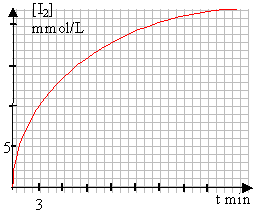
\includegraphics[width=0.38\textwidth]{./img/chimie.png}
\end{center}
\end{wrapfigure}

Pour avoir 10 échantillons identiques du mélange réactionnel initial, on répartit celui-ci dans 10 béchers
à raisons de $V$=$21,5 mL$ par bécher. A l'instant $t = 3min$, on ajoute rapidement de la glace au premier
bécher et on dose le diiode formé $(I_2)$ avec une solution $S_4$ de thiosulfate d’ammonium $(2NH_4^+ + {S_2O_3^{2-}}_{(aq)} )$ de concentration
$C_4$=$1,0.10^{-1} mol.L^{-1}$, en présence d'empois d'amidon. Soit $V_{4E}$ le volume de thiosulfate versé
à l'équivalence. Toutes les 3 minutes, on renouvelle l'opération précédente successivement sur le deuxième
puis le troisième bécher ... etc.

\begin{tblr}{c|[dashed]l}
	0.75  & \textbf{4. } Donner les couples Ox/Red des solutions $S_1$ ,$S_2$ et $S_4$.\\
	1  & \textbf{5. } Ecrire les deux équations relatives à la formation de diiode et au dosage de cette espèce.  \\
	0.75  & \textbf{6. }Montrer que la concentration des ions oxonium issus de l’acide utilisé, dans chaque bécher 

	à $t = 0s$ vaut ${[H_3O^+]}_0$=$7,0.10^{-2} mol/L$ \\

	0.25  & \textbf{7. }Expliquer brièvement le rôle des gouttes d’empois d’amidon ajoutées.\\

	0.25  & \textbf{8. }Pourquoi ajoute-t-on de la glace rapidement à l'instant t, dans chaque bécher ?\\
	0.5  & \textbf{9. }Déterminer l’expression de la concentration, du diiode apparu dans un bécher à l'instant t 

	en fonction de $V_{4E}$. \\
\end{tblr}


La relation précédente a permis de déterminer les variations de $[I_2]$ en diiode en fonction du temps t
comme le montre la courbe de la figure  ci-contre.

\begin{tblr}{c|[dashed]l}
	0.5  & \textbf{10. } Déterminer la valeur de $[I_2]_f$ à la fin de la réaction de formation de diiode

	dans le dernier bécher.\\
	0.5 & \textbf{11. }Montrer que la vitesse de formation du diiode est
	donnée par la relation : $V=\frac{d[I_2]}{dt} $ puis 

	calculer sa vitesse à t = 310s.\\
	0.5 & \textbf{12. }Comment évolue cette vitesse au cours du temps ?
Quel est le facteur cinétique 

responsable de cette
variation ?   \\
	0.5 & \textbf{13. } déduire graphiquement $t_{1/2}$  le temps de demi réaction. \\
\end{tblr}

%\hrulefill
%\Large{Physique 13pts/78min}
%\hrulefill\\
\begin{center}
    %\vspace{.60cm}
\hrulefill
\Large{Physique 13pts}
\hrulefill\\
    \emph{Les deux parties sont indépendantes}
\end{center}

\section*{Partie 1 : Etude d’une onde se propageant le long d’une corde \dotfill(6pts) }

Un vibreur provoque à l’extrémité S d’une corde élastique un mouvement vibratoire sinusoïdal
d’équation $y_{S(t)} = a.cos (2.\pi Nt + \phi )$ où a, N et $\phi$ désignent respectivement, l'amplitude, la fréquence et la
phase à l’origine de S. La source S débute son mouvement à l’instant de date $t_0 = 0 s$. 
On néglige toute atténuation de l’amplitude et toute réflexion de l’onde issue de S.

\begin{tblr}{c|[dashed]l}
	0.25  & \textbf{1. } L'onde se propageant le long de la corde est-elle transversale ou longitudinale ? Justifier.\\
	1 & \textbf{2. }A l’instant $t_1$=$2.10^{-2}s$, le point $M_1$ de la corde d’abscisse $x_1$=$10cm$ entre en vibration. 

	Déterminer
la célérité de l’onde se propageant le long de la corde. \\
	\end{tblr}
\textbf{3. }La courbe représentant l’aspect de la corde à un instant t2 est donnée comme suivante : 
\begin{center}
  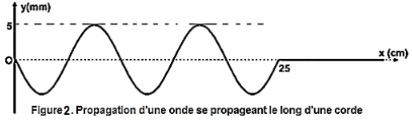
\includegraphics[width=0.7\textwidth]{./img/physique_1.png}
\end{center}
\begin{tblr}{c|[dashed]l}
0.75  & \textbf{3.1. } En exploitant cette courbe, déterminer en unités internationales les valeurs de l’amplitude a ,

la longueur d’onde $\lambda$ et l'instant $t_2$.\\

0.25 & \textbf{3.2. }Déterminer la valeur de la fréquence N.\\

1 & \textbf{3.3. }Déterminer la valeur de la phase initiale $\phi$ de S .\\
1.75 & \textbf{3.4. }Représenter , le diagramme du mouvement du point $M_1$ à la date $t_2$.\\
1 & \textbf{5. }Représenter , le diagramme du mouvement du point $M_1$ à la date $t_2$.
\end{tblr}

\section*{Partie 2 : Etude d’une diffraction \dotfill(7pts) }
On réalise l’expérience de diffraction d’une lumière monochromatique de longueur d’onde $\lambda$ dans le vide
issue d’un appareil laser en utilisant une fente de largeur a et un écran situé à la distance D=1,5m de cette fente .
On obtient le schéma et la courbe de la figure suivante :

\begin{center}
  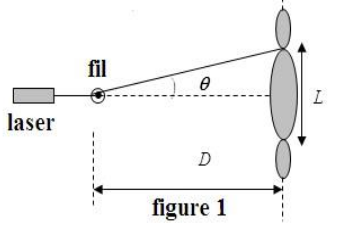
\includegraphics[width=0.3\textwidth]{./img/physique_2.png}
  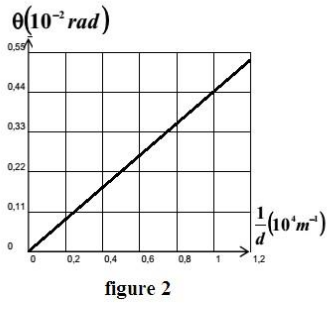
\includegraphics[width=0.3\textwidth]{./img/physique_3.png}
\end{center}

\begin{tblr}{c|[dashed]l}
0.75  & \textbf{1. } Quelle est sa seule caractéristique qui ne change pas quel que soit le
milieu de propagation ?\\

0.25  & \textbf{2. } Décrire la disposition de la fente. Est-elle placée horizontalement ou verticalement ?\\
0.25  & \textbf{3. } Expliquer comment a-t-on trouvé expérimentalement les résultats convertis en graphe 

ci-dessus.\\
0.75  & \textbf{4. }Déterminer l’expression de a en fonction de $\lambda$, D \\
1  & \textbf{5. }Déterminer la valeur de ? est-elle visible ? si oui quelle est sa couleur ?\\
  1 &\textbf{6. }On met maintenant entre la fente et l’écran une lame en plexiglas de forme parallélépipédique 

  comme
le montre la figure  ci-dessous. L’indice de réfraction du verre pour le rayon lumineux

monochromatique utilisé est $n = 1,63$. La tache centrale a pour rayon r’. Déterminer 

l’expression de r’
en fonction de a et n.\\
\end{tblr}

\begin{center}
  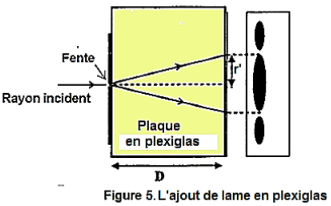
\includegraphics[width=0.34\textwidth]{./img/physique_4.png}
\end{center}

\begin{tblr}{c|[dashed]l}
1  & \textbf{7. } On intercale le diaphragme comportant la fente vers la gauche 

d’une distance $D’= \frac{D}{4}$.
Déterminer l’expression du rayon R de la nouvelle tâche centrale en 

fonction des  paramètres de l’exercice puis déduire l’ordre de grandeur  du rapport $R/r’$. \\
1 & \textbf{8. }Calculer n puis déduire la valeur de la longueur d’onde de la radiation  traversant le plexiglas.\\
1 & \textbf{9. }On enlève la plaque entre la fente et l’écran et on remplace la radiation  monochromatique  par une 

lumière blanche .Expliquer brièvement et avec précision ce qu’on pourrait visualiser sur l’écran.
\end{tblr}

\section*{Vitesse d’onde et tension d’une corde \dotfill(2pts) }
On admet que la vitesse de propagation d’une onde le long d’une corde est liée à la tension de cette corde T et sa masse linéique telle que :  $V = T^{\alpha}.\gamma^{\beta}$..Soit une corde dont l’une des extrémités est fixé , passe
par une gorge et à l’autre extrémité est suspendu un solide de masse m=2,0Kg.La longueur de la corde est
de l=1,60m et sa masse st de m = 20g.

\begin{tblr}{c|[dashed]l}
1  & \textbf{1. } Par les équations aux dimensions donner les valeurs de $\alpha$ et $\beta$.\\
1 & \textbf{2. }Soient deux cordes de même matière. Le diamètre de la première est le double de la deuxième 

mais supporte un solide dont la masse est la moitié du solide suspendue à la première corde. 

Déterminer le rapport $\frac{V_2}{V_1}$

\end{tblr}
\end{document}
